

\section{Implementation}
Most of the theorie behind RS and the methodology it depends on have already been introduced.
The implementation of a RS will be described in the following.
The examples will be written in a programming language called Python.
There is also some SQL code and some UML- and EER-diagrams in order to visualize the concept.

\subsection{Content based RS in-depth}
\label{sec:implementation-contentbased}
The general framework for a content-based RS is shown in figure~\ref{fig:framework-contentbasedrs}.
There are three main components a content-based RS needs.
\begin{itemize}
    \item \textbf{Content Analyzer}\\
        Since all items the RS has to work with can potentially be unstructured, a pre-process is necessary to filter relevant information.
        This will be mainly done by techniques of IR.
        The Content Analyzer aims to bring all items in a from that can be used by its successional components.
        \citep[p.~75-77]{lops:2011}
    \item \textbf{Profile Learner}\\
        When the items are in a suitable form, the Profile Learner can construct a user profile.
        In case of Rocchio's algorithm this includes to distinguish all relevant items from non-relevant.
        With the items and the users preferences the Profile Learner can build the user profile.
        In case of Rocchio, the user profile is a vector representing his attitude towards the different attributes a item may have.
        \citep[p.~75-77]{lops:2011}
    \item \textbf{Filtering Component}\\
        For each user profile the Filtering Component can find items that may match the users preferences.
        Depending on the method implemented the result can be a binary or continuous relevance judgment.
        The continuous relevance judgement is a list of ranked items.
        \citep[p.~75-77]{lops:2011}
        The RS implemented for this thesis uses the k-nearest-neighbours (kNN) classification.
        This results in a list of ranked items where the $k$ best-ranked items will be suggested to the user.
\end{itemize}


\begin{figure}[h]
    \center
    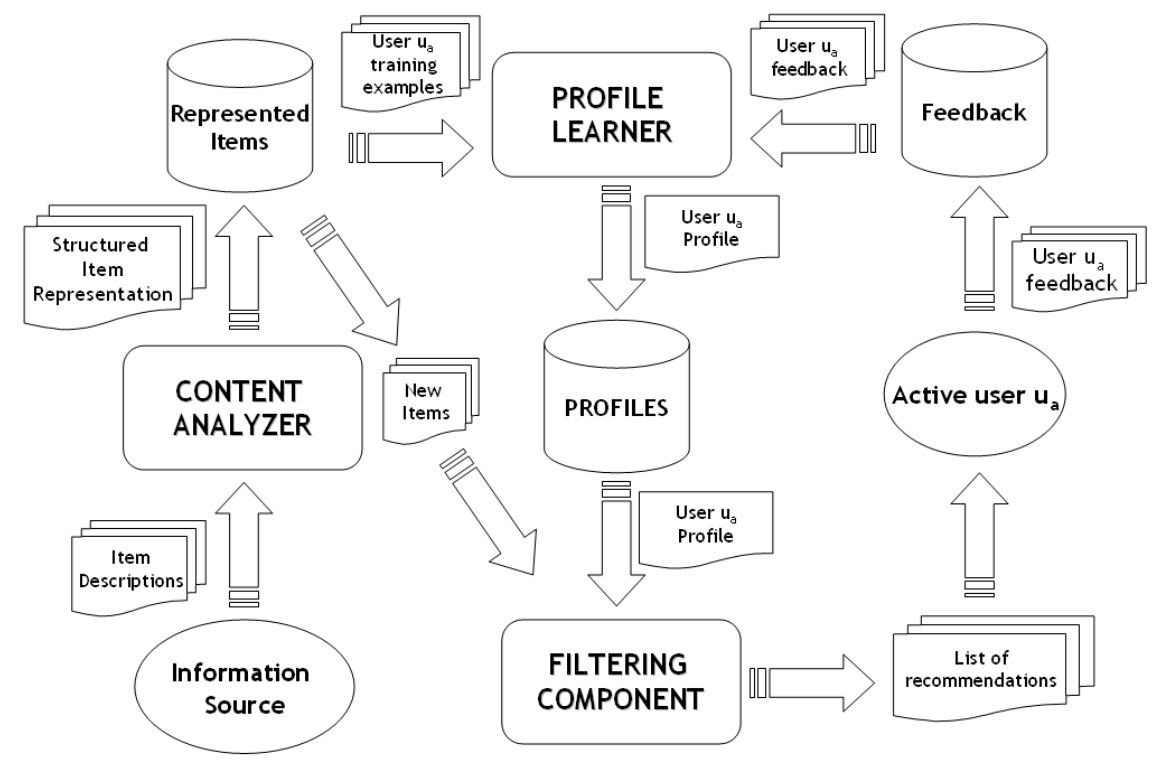
\includegraphics[scale=0.3]{inc/implementation/HighlevelContentBased}
    \caption{High level description of a content-based RS.\citep[p.~76]{lops:2011}}
    \label{fig:framework-contentbasedrs}
\end{figure}



\subsection{Content Analyzer}
\label{sec:content-analyzer}
\index{Content Analyzer}
%{Building the vectors}
%{Storage within the database}
For this project the data describing the products, offered by an online shop have been semi-structured.
It was a text file where each line described a product.
An example is given in listing~\ref{lst:product-data}.

\begin{lstlisting}[caption={Example product data},label={lst:product-data}
    ,keywordstyle=\color{black}
    ,commentstyle=\itshape\color{black}
    ,identifierstyle=\color{black}
    ,stringstyle=\color{black}
]
ImgURL Brand Product Price Shoulder_Width Model_Length Collar_Type Material
http://i1.ztat.net/large/4E/M2/1E/00/0K/11/4EM21E000-K11@4.jpg Emoi en Plus Bluse - dazzling blue 24,95 °(\euro{})° 50 cm 70 cm bei Gr°(\"{o}\ss{})°e 44 Rundhals 100% Polyester
http://i2.ztat.net/large/NA/52/1D/03/NA/11/NA521D03N-A11@3.jpg NAF NAF WENT - Bluse - ecru/noir 38,95 °(\euro{})° 55 cm bei Gr°(\"o{}\ss{})°e S Rundhals 64% Viskose, 22% Baumwolle, 10% Modal, 4% Polyamid
\end{lstlisting}

\noindent
Since the structure of the input was known, it was possible to filter out all relevant product information without using too fancy IR methods.
With regular expressions all relevant informations such as the product\_image-url, brand, product, price, collar type and material have been extracted and stored in a database.
Since a RS could theoretically handle any kind of item afar from products, a distinction has been made between documents in general and products.
The relation between a product and a document has been illustrated in figure~\ref{fig:ertermdocumentassignment}.
It is notable that all terms in a document are treated equally.
This means, that there are no parametric zones or such (section~\ref{sec:parametricandzoneindices}).
\begin{figure}[h]
    \center
    \includegraphics[scale=0.5]{inc/implementation/contentanalyzer/er_term_document_assignment}
    \caption{ER diagram of documents, products and associated terms}
    \label{fig:ertermdocumentassignment}
\end{figure}
Since the relation between \textit{Product} and \textit{Term} is N to N, an intermediate table is neccessary when transforming the ER-diagram into a relational model.
Therefore the table \textit{TermDocumentAssigner} will be introduced and the relational model will look as follows:

\begin{quote}
    \textbf{Document}{(\underline{document\_id})}\\
    \textbf{Product}{(\underline{document\_id[Document]}, image\_name)}\\
    \textbf{Term}{(\underline{term\_id}, name)}\\
    \textbf{TermDocumentAssigner}{(\underline{document\_id[Document], term\_id[Term]}, count)}\\
\end{quote}
\noindent
Since \textit{TermDocumentAssigner} will be very often used to query all terms of a document, it is useful to make an index on \textit{document\_id}.
Implicitly there will also be one on the combined primary key \textit{document\_id, term\_id}.
The tables, implemented by the RS build for this thesis, filled with example data may look as in table~\ref{tab:tablestermdocumentproduct}.
Table~\ref{tab:tablestermdocumentproduct} will serve as resource for terms and documents to illustrate subsequent examples.\\

\begin{table}

    \center

    % Document
    \rowcolors{1}{\dustRowFirst}{\dustRowSecond}
    \begin{tabular}{ l }
        \rowcolor{\dustRowHead}
        \textbf{Document}\\\hline
        document\_id\\\hline
        1\\
        2\\
        3\\
    \end{tabular}
    \quad
    % Product
    \rowcolors{1}{\dustRowFirst}{\dustRowSecond}
    \begin{tabular}{ l | l }
        \rowcolor{\dustRowHead}
        \multicolumn{2}{ c }{\textbf{Product}}\\\hline
        document\_id    & image\_name\\\hline
        1               & image\_1.png\\
        2               & image\_2.png\\
        3               & image\_3.png\\
    \end{tabular}

    ~\\

    %TermDocumentAssigner
    \rowcolors{1}{\dustRowFirst}{\dustRowSecond}
    \begin{tabular}{ l | l | l }
        \rowcolor{\dustRowHead}
        \multicolumn{3}{c}{\textbf{TermDocumentAssigner}}\\\hline
        document\_id    & term\_id  & count\\\hline
        1               & 1         & 1\\
        1               & 2         & 1\\
        1               & 4         & 1\\
        2               & 1         & 1\\
        2               & 3         & 1\\
        2               & 7         & 1\\
        3               & 4         & 1\\
        3               & 5         & 1\\
        3               & 6         & 1\\
    \end{tabular}
    \quad
    % Term
    \rowcolors{1}{\dustRowFirst}{\dustRowSecond}
    \begin{tabular}{ l | l }
        \rowcolor{\dustRowHead}
        \multicolumn{2}{ c }{\textbf{Term}}\\\hline
        term\_id        & name\\\hline
        1               & blouse\\
        2               & blue\\
        3               & polyester\\
        4               & cotton\\
        5               & green\\
        6               & trouser\\
        7               & white\\
    \end{tabular}
    \caption{Table layout defined by figure~\ref{fig:ertermdocumentassignment}}
    \label{tab:tablestermdocumentproduct}
\end{table}

\noindent
As already mentioned before, Rocchio's algorithm works best with tf-idf vectors.
Since the theory has been described in section~\ref{sec:tfidf}, the next big step is to show how vectors for this project have been built.
A short reminder: currently all products are described through their terms.\\

\noindent
In order to build tf-idf vectors, one also has to built term frequency, as well as inverse document frequency vectors - these are the preconditions.
Since these tasks are fairly similar, some design patterns help realizing them.
The \gls{abstract factory} pattern proofed to be very handy for this task.
For each necessary vector (tf, idf, tf-idf) one can build a vector creator which shares the design of the other vector creators.
Therefore the abstract class \textit{VectorCreator} has been introduced.
The \textit{VectorCreator} offers the abstract method \textit{\_get\_vector(document\_id:int):DocumentVector} which will be responsible for creating all vectors.
All inherited classes will implement the abstract method with a procedure to create an instance of \textit{DocumentVector}.

\paragraph{Term frequency vector}
\index{Term Frequency}
Every term frequency vector representing a document consists of the term frequency of all terms.
The current implementation uses the SQL query displayed in listing~\ref{lst:tf-query} for generating the tf vector.
The result of a query may look as follows (based on the tables shown in figure~\ref{fig:ertermdocumentassignment} and are displayed in table~\ref{tab:tf-query-result}.
\begin{table}
    \rowcolors{1}{\dustRowFirst}{\dustRowSecond}
    \begin{tabular}{ l|l|l || l|l|l || l|l|l }
        \rowcolor{\dustRowHead}
        \multicolumn{3}{c||}{\textbf{$\text{tf}_\text{document\_1}$}} &
        \multicolumn{3}{c||}{\textbf{$\text{tf}_\text{document\_2}$}} &
        \multicolumn{3}{ c }{\textbf{$\text{tf}_\text{document\_3}$}}\\\hline

        term\_id & name & value                          & term\_id & name  & value             & term\_id & name & value\\\hline
        1   & blouse    & 1                              & 1    & blouse    & 1                 & 1 & blouse  & 0\\
        2   & blue      & 1                              & 2    & blue      & 0                 & 2 & blue  & 0\\
        3   & polyester & 0                              & 3    & polyester & 1                 & 3 & polyester  & 0\\
        4   & cotton    & 1                              & 4    & cotton    & 0                 & 4 & cotton  & 1\\
        5   & green     & 0                              & 5    & green     & 0                 & 5 & green  & 1\\
        6   & trouser   & 0                              & 6    & trouser   & 0                 & 6 & trouser  & 1\\
        7   & white     & 0                              & 7    & white     & 1                 & 7 & white  & 0\\
    \end{tabular}
    \caption{Possible result of the query in listing~\ref{lst:tf-query}}
    \label{tab:tf-query-result}
\end{table}

\begin{lstlisting}[language=SQL,caption={SQL query for generating tf-vectors},label={lst:tf-query},float=h]
-- :document_id is a parameter given to the method
SELECT
    [t].[term_id]
    , [t].[name]
    , CASE WHEN  [a].[document_id] IS NULL
        THEN    0
        ELSE    [a].[count]
    END AS [value]
FROM
    [Term] AS [t]
    LEFT OUTER JOIN [TermDocumentAssigner] AS [a]
        ON  [t].[term_id] = [a].[term_id]
        AND [document_id] = :document_id
ORDER BY    [t].[term_id]
;
\end{lstlisting}

\noindent
The result of the query shown in listing~\ref{lst:tf-query} will finally be stored in the \textit{TermFrequencyVector} class derived from \textit{DocumentVector} (see figure~\ref{fig:uml-document-vectors}).

\paragraph{Document frequency vector}
\index{Document Frequency}
In contrast to the \textit{TermFrequencyVector} the \textit{DocumentFrequencyVector} does not resemble a single document, rather than the whole collection of documents.
Therefore the parameter \textit{document\_id} can be omitted.
But in order to sustain uniformity between all classes inheriting from \textit{VectorCreator} it will be carried along but set to a null value.
To make the source code more readable, the SQL code for querying the document-frequency values has been outsourced to a SQL-View as shown in listing~\ref{lst:df-view}.
This little tweak (that has no influence on speed) left the query for df-vectors as simple as shown in listing~\ref{lst:df-query}.
The result for the example is given in table~\ref{tab:df-query-result}.

\begin{lstlisting}[language=SQL,caption={SQL statement to create the \textit{DocumentFrequency}-view},label={lst:df-view},float=h]
CREATE VIEW IF NOT EXISTS [DocumentFrequency] AS
    SELECT
            [t].[term_id]
            , [t].[name]
            , CASE WHEN   [a].[count] IS NULL
                THEN        0
                ELSE        [a].[count]
            END AS [value]
    FROM
        [Term] as [t]
        LEFT OUTER JOIN
        (
            SELECT
                [term_id]
                , SUM([document_id]) AS [count]
            FROM
                [TermDocumentAssigner]
            GROUP BY
                [term_id]
        ) AS [a]
            ON [t].[term_id] = [a].[term_id]
    ORDER BY
        [t].[term_id]
;
\end{lstlisting}

\begin{lstlisting}[language=SQL,caption={SQL query for generating df-vectors},label={lst:df-query},float=h]
SELECT
    [term_id]
    , [name]
    , [value]
FROM
    [DocumentFrequency]
;
\end{lstlisting}

\begin{table}
    \center
    \rowcolors{1}{\dustRowFirst}{\dustRowSecond}
    \begin{tabular}{ l | l | l }
        \rowcolor{\dustRowHead}
        \multicolumn{3}{ c }{\textbf{df}}\\\hline
        term\_id    & name      & value\\\hline
        1           & blouse    & 2\\
        2           & blue      & 1\\
        3           & polyester & 1\\
        4           & cotton    & 2\\
        5           & green     & 1\\
        6           & trouser   & 1\\
        7           & white     & 1\\
    \end{tabular}
    \caption{Possible results of the query in figure~\ref{lst:df-query}}
    \label{tab:df-query-result}
\end{table}

\begin{figure}[h]
    \center
    \includegraphics[scale=0.4]{inc/implementation/contentanalyzer/uml_document_vectors}
    \caption{Document vectors}
    \label{fig:uml-document-vectors}
\end{figure}

\paragraph{Inverse document frequency vector}
\index{Inverse Document Frequency}
For building idf-vectors one can use df-vectors (and their source code) as basis.
The inverse document frequency is calculated by dividing the total count of documents in a collection through the document frequency of a term.
Another SQL-View called N-view will provide the number of documents, while the code for creating idf-vectors get outsourced into its own view once more.
Since the SQL implementation of \gls{sqlite3} does not offer a logarithm-function, one has to defined his very own.
Fortunately the standard python library for connecting to sqlite3-databases supports the creation of functions as shown in listing~\ref{lst:idf-view}.


\begin{lstlisting}[language=Python,caption={SQL-statement to create the InverseDocumentFrequency-view},label={lst:idf-view}]
def _create_log_function(self, conn):
    conn.create_function('log10', 1, InverseDocumentFrequencyVectorCreator.log_10)
    pass

def log_10(x):
    base = 10
    return math.log(x, base)
\end{lstlisting}
\begin{lstlisting}[language=SQL]
CREATE VIEW IF NOT EXISTS [InverseDocumentFrequency] AS
    SELECT
        [term_id]
        , [name]
        , log10
        (
            CAST ((SELECT [document_count] from [N]) AS REAL) / [df].[value]
        )
         AS [value]
    FROM
        [DocumentFrequency] AS [df]
    ORDER BY
        [term_id]
    ;
\end{lstlisting}


\begin{lstlisting}[language=SQL,caption={SQL-statement to create the N-view},label={lst:n-view},float=h]
CREATE VIEW IF NOT EXISTS [N] AS
    SELECT
        (SELECT COUNT(*) FROM [Document]) AS [document_count]
        , (SELECT COUNT(*) FROM [Term]) AS [term_count]
;
\end{lstlisting}


\begin{lstlisting}[language=SQL,caption={SQL-query for generating idf-vectors},label={fig:idf-query},float=h]
SELECT
    [term_id]
    , [name]
    , [value]
FROM
    [InverseDocumentFrequency]
;
\end{lstlisting}


\begin{table}
    \center
    \rowcolors{1}{\dustRowFirst}{\dustRowSecond}
    \begin{tabular}{ l | l | l }
        \rowcolor{\dustRowHead}
        \multicolumn{3}{ c }{\textbf{idf}}\\\hline
        term\_id    & name      & value\\\hline
        1           & blouse    & $\log_{10}(3/2) \approx 0.18$\\
        2           & blue      & $\log_{10}(3/1) \approx 0.48$\\
        3           & polyester & $\log_{10}(3/1) \approx 0.48$\\
        4           & cotton    & $\log_{10}(3/2) \approx 0.18$\\
        5           & green     & $\log_{10}(3/1) \approx 0.48$\\
        6           & trouser   & $\log_{10}(3/1) \approx 0.48$\\
        7           & white     & $\log_{10}(3/1) \approx 0.48$\\
    \end{tabular}
    \caption{Possible results of the query in figure~\ref{fig:idf-query}}
    \label{tab:idf-query-result}
\end{table}

\paragraph{Tf-idf vector}
\index{TfIdf}
Finally one can create tf-idf vectors which are the combination of tf- and idf-vectors (as explained in section~\ref{sec:tfidf}).
Since tf-idf is merely the multiplication of term frequency with the corresponding inverse document frequency, it's rather simple to calculate.
Listing~\ref{lst:tfidf-code} shows the creation of a \textit{TfIdfVector} in the method \textit{\_create\_vector()}, whereas the multiplication is in method \textit{\_get\_values()}.

\begin{lstlisting}[language=Python,caption={Python code for calculating tfidf-vectos on basis on tf- and idf-vectors},label={lst:tfidf-code},float=h]
class TfIdfVectorCreator(VectorCreator):

    def __init__(self, db_connection_str):
        super(TfIdfVectorCreator, self).__init__(db_connection_str)

        self._tf_creator = TermFrequencyVectorCreator(db_connection_str)
        self._idf_creator = InverseDocumentFrequencyVectorCreator(db_connection_str)
        pass

    def _create_vector(self, document_id):
        tf_vector = self._tf_creator.get_vector(document_id)
        idf_vector = self._idf_creator.get_vector(document_id)

        tfidf_vector = TfIdfVector()

        for triple in self._get_values(tf_vector, idf_vector):
            tfidf_vector.add_to_vector(triple)

        return tfidf_vector

    def _get_values(self, tfv, idfv):
        ingredients = zip(tfv.term_id, tfv.description, tfv.values, idfv.values)

        for (tf_tid, tf_desc, tf_val, idf_val) in ingredients:
            yield (tf_tid, tf_desc, tf_val * idf_val)
            pass
        pass
\end{lstlisting}

\begin{table}
    \rowcolors{1}{\dustRowFirst}{\dustRowSecond}
    \begin{tabular}{ l|l|l || l|l|l || l|l|l }
        \rowcolor{\dustRowHead}
        \multicolumn{3}{c||}{\textbf{$\text{tf-idf}_\text{document\_1}$}} &
        \multicolumn{3}{c||}{\textbf{$\text{tf-idf}_\text{document\_2}$}} &
        \multicolumn{3}{ c }{\textbf{$\text{tf-idf}_\text{document\_3}$}}\\\hline

        term\_id & name & value             & term\_id & name & value           & term\_id & name & value\\\hline
        1   & blouse    & $\approx 0.18$    & 1    & blouse   & $\approx 0.18$  & 1 & blouse      & 0\\
        2   & blue      & $\approx 0.48$    & 2    & blue     & 0               & 2 & blue        & 0\\
        3   & polyester & 0                 & 3    & polyester& $\approx 0.48$  & 3 & polyester   & 0\\
        4   & cotton    & $\approx 0.18$    & 4    & cotton   & 0               & 4 & cotton      & $\approx 0.18$\\
        5   & green     & 0                 & 5    & green    & 0               & 5 & green       & $\approx 0.48$\\
        6   & trouser   & 0                 & 6    & trouser  & 0               & 6 & trouser     & $\approx 0.48$\\
        7   & white     & 0                 & 7    & white    & $\approx 0.48$  & 7 & white       & 0\\
    \end{tabular}
    \caption{Possible result of the function in figure~\ref{lst:tfidf-code}}
    \label{tab:tfidf-query-result}
\end{table}


With the vectors built, the main task of the content analyzer is done.
However there is still one more enhancement one can implement to make the repetitive creation of vectors faster.
Through dynamic (for details see section~\ref{sec:dynamic-programming}) programming we can easily "re-create" vectors we already used once.
Since it proves useful, if all inheriting classes of \textit{VectorCreator} can use dynamic programming without explicitly implementing it, one can implement the \textit{VectorCreator} as proxy (explained in sectin~\ref{sec:proxy}).
As a result the \textit{VectorCreator} gets another method called \textit{get\_vector(document\_id:int)} to which the same rules apply as to \textit{\_create\_vector(document\_id:int)}.
The buffering of \textit{DocumentVectors} can now be implemented in \textit{get\_vector(document\_id:int)} and all inheriting classes will also posses caching capabilities.
The code for dynamic programming is shown in listing~\ref{lst:dynamic-programming}.\\
In order to get a picture of all important vectors and their creation, a UML-diagram has been included (figure~\ref{fig:uml-vectorssimple}).

\begin{lstlisting}[language=Python,caption={Dynamic programming},label={lst:dynamic-programming},float=h]
class VectorCreator(object):

    # ... omitted unnecessary code

    def get_vector(self, document_id=None):
        if document_id is not None and not isinstance(document_id, int):
            raise TypeError('document_id must either be an integer or None')
        if not document_id in self._cache:
            vector = self._create_vector(document_id)
            if vector.document_id is None:
                vector.document_id = document_id
            self._cache[document_id] = vector
        return self._cache[document_id]}

    def _create_vector(self, document_id):
        # ... creating vector
\end{lstlisting}


\begin{figure}[h]
    \center
    \includegraphics[scale=0.33,angle=90]{inc/implementation/contentanalyzer/uml_vectors_simple}
    \caption{Abstract and concrete vector fabric}
    \label{fig:uml-vectorssimple}
\end{figure}

\FloatBarrier

\subsection{Profile Learner}
%{Rocchio algorithm}
%{Relevance feedback}
With the products in a database and being capable to form them into vectors, the next step is to implement the profile learner.
As already mentioned the algorithm of choice is Rocchio's algorithm (introduced in section~\ref{sec:rocchio}).
It creates a user vector that gets refined every time the user gives feedback about his preferences.
Therefore a new table that holds the user vector is necessary.
Furthermore one has to store the users feedback towards some of the documents.
The er-diagram in figure~\ref{fig:er_user_table} shows the layout which has been implemented.\\
Each user is identified by an unique id (\textit{user\_id}) and optionally by a also unique name (\textit{name}).
Any user can specify his preferences by marking some documents as relevant.
This will be further explained when discussing the possibilities of user feedback.
{\color{red}TODO}
Because the algorithm can work with any of the stored items, it rather works on \textit{Documents}, than on \textit{Products}.
For each of the terms which define a document the user has a "value" that defines his attitude towards the term.
The more similar the users value of a term $t$ is with a $\text{tf-idf}_t$ value of a document, the more likely he can can make use of the document/product.
The users position towards a term is stored within the relation between the user and the corresponding term.

% user vector creator and uservector
\begin{figure}[h]
    \center
    \includegraphics[scale=0.5]{inc/implementation/profilelearner/er_user_table}
    \caption{ER diagram of user and his related entities}
    \label{fig:er_user_table}
\end{figure}

\noindent
When forming the er diagram in figure~\ref{fig:er_user_table} into a relational schema the result will look like below.
Whereas the user is represented by \textit{User}, the N-to-N relation between \textit{User} and \textit{Document} will be solved by a new table \textit{UserPreference} and the relationship between \textit{User} and \textit{Term} with a attribute becomes \textit{UserVector}.
\begin{quote}
    \textbf{User}($\underline{\text{user\_id}}$, name)\\
    \textbf{UserPreference}($\underline{\text{user\_id[userManagement]},\text{document\_id[Document]}}$)\\
    \textbf{UserVector}($\underline{\text{user\_id[UserManagement], term\_id[Term]}}$, value)\\
\end{quote}

% user vector
\begin{figure}[h]
    \center
    \includegraphics[scale=0.3]{inc/implementation/profilelearner/uml_vector_user}
    \caption{UML diagram describing UserVector and UserVectorCreator}
    \label{fig:uml_vector_user}
\end{figure}

\begin{lstlisting}[language=SQL,caption={SQL query for creating a user vector},label={lst:user-vector-query},float=h]
SELECT
    [t].[term_id]
    , [t].[name]
    , [uv].[value]
FROM
    [Term] AS [t]
    JOIN [UserVector] AS [uv]
        ON [t].[term_id] = [uv].[term_id]
WHERE
    [uv].[user_id] = :user_id
ORDER BY
    [t].[term_id]
;
\end{lstlisting}

\begin{table}
    \rowcolors{1}{\dustRowFirst}{\dustRowSecond}
    \begin{tabular}{ l | l }
        \rowcolor{\dustRowHead}
        \multicolumn{2}{c}{\textbf{User}}\\\hline
        user\_id    & name \\\hline
        1           & user\_test\\
    \end{tabular}
    \quad
    \rowcolors{1}{\dustRowFirst}{\dustRowSecond}
    \begin{tabular}{ l | l }
        \rowcolor{\dustRowHead}
        \multicolumn{2}{c}{UserPreference}\\\hline
        user\_id    & document\_id\\\hline
        1           & 2\\
    \end{tabular}
    \quad
    \rowcolors{1}{\dustRowFirst}{\dustRowSecond}
    \begin{tabular}{ l | l | l }
        \rowcolor{\dustRowHead}
        \multicolumn{3}{c}{UserVector}\\\hline
        user\_id    & term\_id  & value\\\hline
        1           & 1         & 0\\
        1           & 2         & 0\\
        1           & 3         & 0\\
        1           & 4         & 0\\
        1           & 5         & 0\\
        1           & 6         & 0\\
        1           & 7         & 0\\
    \end{tabular}
    \caption{User table and dependencies filled with example values}
    \label{tab:user}
\end{table}

\noindent
Listing~\ref{lst:rocchio} finally displays the implementation of Rocchio's algorithm.
Based on the example set up in section~\ref{sec:content-analyzer}, there is an example how the algorithms changes user vectors.\\
Parameter \textit{q\_0} of function \textit{calculate()} is the current vector that represents the user.\\
Rocchio's algorithm will create a new vector that refines and replaces the current one.
\textit{list\_d\_related} is a list of related documents (the terminology is derived from information retrieval).
Any document that the user marked as preferences counts as relevant.\\
A list of all irrelevant documents will be passed via \textit{list\_d\_unrelated}.\\
It is possible to either use pre-defined weightings for the variables $\alpha$, $\beta$, or $\gamma$, represented by "a", "b" and "c".
But of course the user of the library can also define his very own weights by passing a triple as fourth parameter to the function \textit{calculate}.
When no weights are passed explicitly, the function will call \textit{default\_weights()} in order to gain the pre-set default values.
Based on the weights the result for refined user vector will vary greatly.\\
The return value \textit{q\_m} finally is the updated user vector that must replace the vector stored in table \textit{UserVector}.
When this is done, one has successfully used Rocchio's algorithm to adopt a user vector to the users feedback.
An example is given below.

\begin{lstlisting}[language=Python,caption={Implementation of Rocchio's algorithm},label={lst:rocchio},float=h]
def default_weights():
    a = 1
    b = 0.85
    c = 0.15
    return (a, b, c)

def calculate(q_0, list_d_related, list_d_unrelated, weights=default_weights()):
    a, b, c = weights

    def calculate_a():
        return q_0.scalar_multiplication( a )

    def calculate_b():
        if len(list_d_related) > 0:
            return (
                    sum(list_d_related)
                    .scalar_multiplication(1/len(list_d_related))
                ).scalar_multiplication(b )
        return null_vector()

    def calculate_c():
        if len(list_d_unrelated) > 0:
            return (
                    sum(list_d_unrelated)
                    .scalar_multiplication(1/len(list_d_unrelated))
                ).scalar_multiplication(c)
        return null_vector()

    def null_vector():
        empty = q_0.scalar_multiplication(0)
        return empty
        
    q_m = calculate_a() + calculate_b() - calculate_c()
    return q_m
\end{lstlisting}

\noindent
Assuming that the user also likes document 1 and therefore gives the RS feedback about document 1, Rocchio's algorithm would work as shown in the equation below (based on the values in table~\ref{tab:user} and \ref{tab:idf-query-result}).
By comparing $\text{q}_0$ with the modified vector $\text{q}_\text{m}$ one can see in which way the vector has changed (the initial vector $\text{q}_0$ has been set to this value by default).
\begin{align*}
    \alpha &= 1;\quad \beta = 0.85;\quad \gamma = 0.15\\
    \text{q}_0 &= (0, 0, 0, 0, 0, 0, 0)^T \\
    \text{l}_\text{dr} &= \{(0.18, 0.48, 0, 0.18, 0, 0, 0)^T, (0.18, 0, 0.48, 0, 0, 0, 0, 0.48)^T\}\\
    \text{l}_\text{dnr} &= \{(0, 0, 0, 0, 0.18, 0.48, 0.48, 0)^T\}\\
    \text{q}_\text{m} &=
        \alpha \cdot \text{q}_0
        + \beta \cdot \frac{1}{|\text{l}_\text{dr}|}\sum_{\text{d}_\text{j}\in\text{l}_\text{dr}}\vec{\text{d}}_\text{j}
        - \gamma \cdot \frac{1}{|\text{l}_\text{dnr}|}\sum_{\text{d}_\text{j}\in\text{l}_\text{dnr}}\vec{\text{d}}_\text{j}\\
    &= 1 \cdot (0, 0, 0, 0, 0, 0, 0)^T\\
        &\quad+ 0.85 \cdot \frac{1}{2} \cdot \big((0.18, 0.48, 0, 0.18, 0, 0, 0)^T+(0.18, 0, 0.48, 0, 0, 0, 0, 0.48)^T \big)\\
        &\quad- 0.15 \cdot \frac{1}{1} \cdot(0, 0, 0, 0, 0.18, 0.48, 0.48, 0)^T\\
    &= (0, 0, 0, 0, 0, 0, 0)^T\\
        &\quad+(0.153, 0.204, 0.204, 0.0765, 0, 0, 0.204)^T\\
        &\quad-(0, 0, 0, 0.027, 0.072, 0.072, 0)^T\\
    &= \underline{\underline{
            (0.153, 0.204, 0.204, 0.0495, -0.072, -0.072, 0.204)^T
        }}
\end{align*}

\FloatBarrier

\subsection{Filtering Component}
%%%%%%%%%%%%%%%%%%%%%%%%%%
%k nearest neighbours
% manning 297, 290 (euclidean distance)
%%%%%%%%%%%%%%%%%%%%%%%%%%
\index{filtering component}
\label{sec:filtering-component}
{\color{red}\tiny Discuss euclidean and hamming distance}
As filtering component $k$ nearest neighbours (kNN) has been implemented.
One of its advantages is, that it does not require any training or whatsoever.\citep[p.~290]{manning:2009}
kNN will return a list of the $k$ closest vectors around a given centroid.
Therefore $k$ can be interpreted as a parameter.
When the value for $k$ is already determined (for instance $k=3$), than one can also speak of 3NN.\citep[p.~297-298]{manning:2009}
To measure distance between two vectors the algorithm relies on the Euclideans distance, as is has been suggested by \citeauthor{manning:2009}.\citep[p.~292]{manning:2009}
For comparision other ways for calculating the distance have also been implemented - namely the Hamming distance.
When using kNN it is recommended to choose a value $k > 1$, since otherwise it is deemed as not robust.
It's also better to choose an odd value for $k$.\\
An implementation of $k$NN with exchangeable distance function is displayed in listing~\ref{lst:knn}.

\begin{lstlisting}[language=Python,caption={kNN and distance methods},label={lst:knn},float=h]
def hamming_distance(v1, v2):
    return v1.hamming_distance(v2)

def euclidean_distance(v1, v2):
    return v1.euclidean_distance(v2)

default_distance = euclidean_distance

def k_nearest_neighbours(k, vector_origin, vectors, distance_function=default_distance):
    distances = [(distance_function(vector_origin, v), v) for v in vectors]
    ratings = distances
    ratings.sort()  # sorts ascending by distance, then by DocumentVector
    return [(r, v) for (r, v) in ratings[:k] ]

class DocumentVector(object):

    # ... omitted uneccesary code

    def hamming_distance(self, other):
        distance = 0
        for val1, val2 in zip(self.values, other.values):
            if not val1 == val2:
                distance += 1
        return distance

    def euclidean_distance(self, other):
        t = sum(
            ((v1 - v2) ** 2  for v1, v2 in zip(self.values, other.values))
        )
        d = math.sqrt(t)
        return d
\end{lstlisting}

The \textit{k\_nearest\_neighbours} function awaits a $k$ as first parameter, specifying the size of the list to return.
As second parameter the function gets a vector which suits as fixpoint for calculating the distances called \textit{vector\_origin}.
\textit{vectors} are all vectors whose distance shall be measured.
As an optional argument \textit{k\_nearest\_neighbours} awaits a function for calculating the distance.
Per default, the function is \textit{euclidean\_distance} which calculates the euclidean distance between two vectors.

When using this $k$NN with the euclidean distance function on the data of the example, the results will look as in the table~\ref{tab:knn-result}.
As parameter $k$ 2 has been chosen.



\begin{table}
    \center
    \rowcolors{1}{\dustRowFirst}{\dustRowSecond}
    \begin{tabular}{ l | l | l }
        \rowcolor{\dustRowHead}
        rank    & distance              & document\_id\\\hline
        1       & 0.43305340317332686   & 1\\
        2       & 0.45553841769931985   & 2\\
        %3       & 0.8801677396951105    & 3\\
    \end{tabular}
    \caption{Possible $k$NN result for $k=2$}
    \label{tab:knn-result}
\end{table}

\FloatBarrier


\section{Web-API}
\label{sec:web-api}
The whole library bundling the recommender system logic is written in Python, it is hard to use it from any other programming language except for Python.
Since this is a major drawback there is a additional \gls{web api} that creates a server which uses the recommender library and forwards all method calls.
The web API offers methods for all frequently performed tasks.
As data format for transfering information \textit{\gls{json}} will be used.
Many programming languages offer native support for interpreting JSON.
{\color{red}JSON}

\begin{description}
    \item[\textit{GET} /product/get/\textless product\_id\textgreater]\hfill\\
        foobar
    \item[\textit{GET} /product/all]\hfill\\
        foobar
    \item[GET /product/random/\textless count\textgreater]\hfill\\
        foobar
    \item[\textit{POST} /product/insert]\hfill\\
        curl -X POST -d "product=\{'image\_name':'img.jpg','terms':\{'a':1,'b':3\}\}"
    \item[\textit{GET} /vector/default/\textless doc\_id\textgreater]\hfill\\
        foobar
    \item[\textit{GET} /vector/df]\hfill\\
        foobar
    \item[\textit{GET} /vector/idf]\hfill\\
        foobar
    \item[\textit{GET} /vector/tf/\textless doc\_id\textgreater]\hfill\\
        foobar
    \item[\textit{GET} /vector/tfidf/\textless doc\_id\textgreater]\hfill\\
        foobar
    \item[\textit{GET} /vector/user/\textless user\_id\textgreater]\hfill\\
        foobar
    \item[\textit{GET} /vector/user/\textless user\_name\textgreater]\hfill\\
        foobar
    \item[\textit{GET} /user/all]\hfill\\
        foobar
    \item[\textit{GET} /user/create/\textless user\_name\textless]\hfill\\
        foobar
    \item[\textit{GET} /user/exists/\textless user\_name\textgreater]\hfill\\
        foobar
    \item[\textit{GET} /user/createifnotexist/\textless user\_name\textgreater]\hfill\\
        foobar
    \item[\textit{GET} /user/setpreference/\textless user\_name\textgreater /\textless produc\_id\textgreater]\hfill\\
        foobar
    \item[\textit{GET} /user/setpreference/\textless user\_name\textgreater /\textless produc\_id\textgreater]\hfill\\
        foobar
    \item[\textit{GET} /user/update/\textless user\_name\textgreater]\hfill\\
        foobar
    \item[\textit{GET} /user/relevant/\textless user\_name\textgreater]\hfill\\
        foobar
    \item[\textit{GET} /user/norelevant/\textless user\_name\textgreater]\hfill\\
        foobar
    \item[\textit{GET} /recommendations/\textless user\_name\textgreater /\textless k\textgreater]\hfill\\
        foobar


\end{description}

\FloatBarrier

\subsection{Online shop}
As already mentioned in previous sections it is not the goal to implement a fully functional online shop as one may know it from Amazon.com or similiar vendors.
Instead this one focuses on offering products, collecting feedback from the user and finally generating recommendations which will be presented to the user.

\subsubsection{General look and feel}
The key functionality of given an overview of items and recommendations is being displayed in figure~\ref{fig:onlineshop-overview}.
While random products are displayed in the left column, possible recommendations will be displayed in the right colum which is highlighted in light green.
As soon as one clicks on one of the items displayed a product view will be opened where most of the information about the selected product will be available.
The product view is responsible for receiving and interpreting the users feedback and will be further explained in section~\ref{sec:onlineshop-feedback}.

\begin{figure}[h]
    \center
    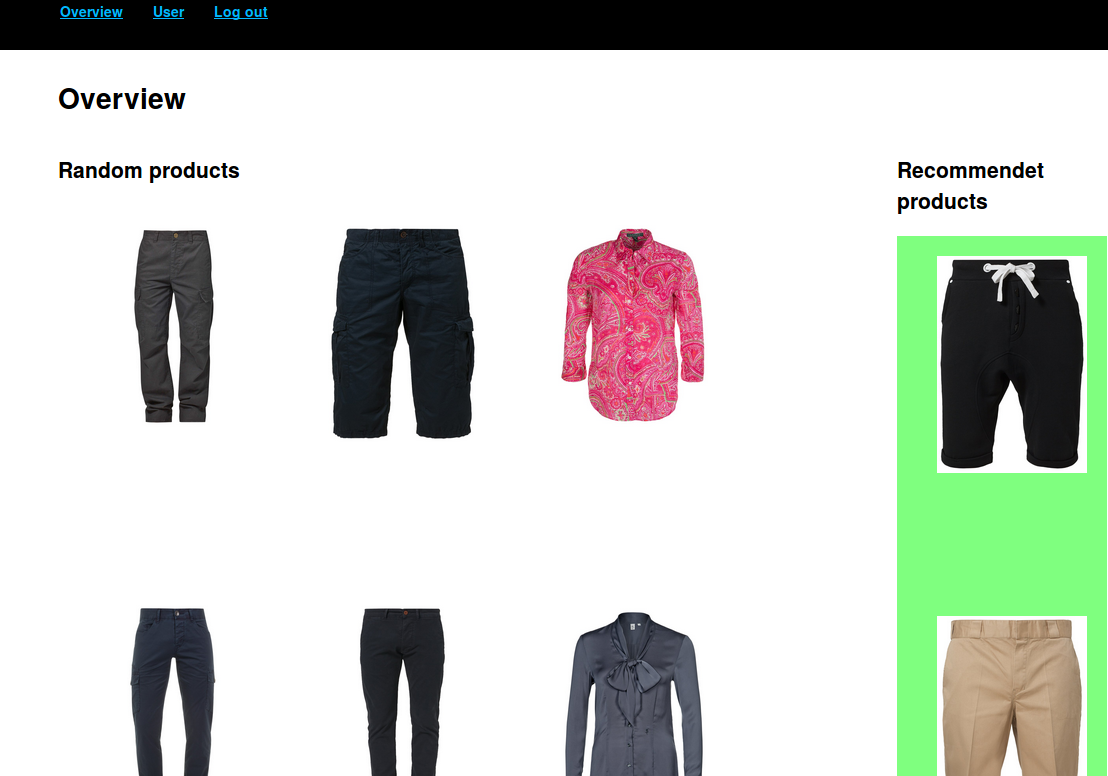
\includegraphics[scale=0.3]{inc/implementation/onlineshop/recommender_onlineshop_overview}
    \caption{Online shop overview}
    \label{fig:onlineshop-overview}
\end{figure}

\subsubsection{Feedback}
\label{sec:onlineshop-feedback}
Both implicit and explicit feedback as introduced in section~\ref{sec:feedback} have been implemented.
Even thought the initial task was to implement a RS that utilizes implicit feedback, explicit has been implemented as well to compare both methods.
There are three different ways of collecting feedback used by the online shop.
\begin{itemize}
    \item \textbf{Implicit}\hfill\\
        Whenever the user selects an item from the online-shops overview this will be interpreted as positive feedback towards the item.
    \item \textbf{Implicit timed}\hfill\\
        Instead of interpreting every item the user examines as explicit indicator for sympathy towards the product it will be measured how long the user views the product.
        It is assumed, that if the user still views the product after a pre-determined period of time he might be interessted in this particular item.
    \item \textbf{Explicit binary rating}\\
        The product-view will be equiped with a binary rating component which enables the user to explicitely like or dislike an item.
        This allows the user to remove items from the list of liked items which is not possible for the prior listed implicit methods since the user couldn't actively dislike an item.
\end{itemize}

Since implicit feedback do not require any interaction with a user there is no user interface with which a user can interact.
For explicit feedback however the user has been given the opportunity to give a binary rating about a item whether he likes it or not.
A snippet of the user interace for explict rating is shown in figure~\ref{fig:onlineshop-explicit-rating}.

\begin{figure}[h]
    \center
    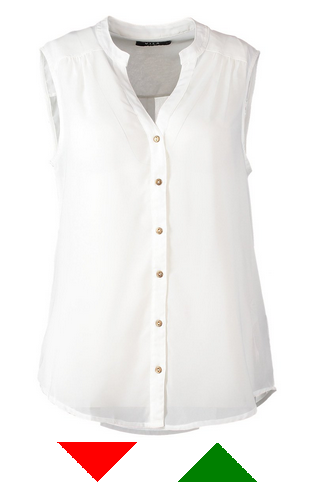
\includegraphics[scale=0.3]{inc/implementation/onlineshop/recommender-onlineshop-binary_rating}
    \caption{Binary rating of an item}
    \label{fig:onlineshop-explicit-rating}
\end{figure}


\subsubsection{Differences to real onine shops}
Even thought there are major differences between the implemented online shop and

%tracking through cookies

\FloatBarrier


\subsection{Derp}
Umfang und Aufgaben der Lib erkl\"aren.

\subsection{Testing and findings}
wie sind die Empfehlungen des algorithmus
